\documentclass[tikz]{standalone}
\usepackage{mwe}
\usepackage{lipsum}
\usepackage{relsize}
\usetikzlibrary{positioning	}
\usetikzlibrary{arrows.meta}
% Macros
\newcommand{\xo}{\bigotimes}

%%%%%%%%%%%%%%%%%%%%%%%%%%%%%%%%%%%%%%%%%%%%%%%%%%%%%%%%%%%%%%%%%%%%%%%%%%%%%%%%%%%%%%%%
% Poster parameters %%%%%%%%%%%%%%%%%%%%%%%%%%%%%%%%%%%%%%%%%%%%%%%%%%%%%%%%%%%%%%%%%%%%
%%%%%%%%%%%%%%%%%%%%%%%%%%%%%%%%%%%%%%%%%%%%%%%%%%%%%%%%%%%%%%%%%%%%%%%%%%%%%%%%%%%%%%%%

% Colours
\newcommand{\macrocolor}{red}
\newcommand{\microcolor}{blue}
\newcommand{\macrotext}[1]{\color{\macrocolor}#1}
\newcommand{\microtext}[1]{\color{\microcolor}#1}

% Graph box parameters
\newcommand{\FIGWIDTH}{15cm} % figure width
\newcommand{\FIGHEIGHT}{11cm} % figure height
\newcommand{\VERTFIGSEP}{5cm} % vertical separation between figures
\newcommand{\HORFIGSEP}{6cm} % horizontal separation between figures

% Axis box and line style
\tikzstyle{axisbox} = [inner sep=0]
\tikzstyle{axisline} = [
		% {Latex[length=1cm, width=1cm]}-{Latex[length=1cm, width=1cm]},
		-{Latex[length=1cm, width=1cm]},
		ultra thick,
		>=stealth
]

% Model point style
\tikzstyle{modelpoint} = [
		circle,
		fill=black,
		inner sep=0pt,
		minimum size=0.5cm,
		prefix after command= {\pgfextra{\tikzset{every label/.style={font=\Huge}}}}
]

% Textbox style
\tikzstyle{mybox} = [
		draw=red,
		fill=blue!20,
		very thick,
    rectangle,
		rounded corners,
		inner sep=10pt,
		inner ysep=20pt]
\tikzstyle{fancytitle} = [fill=red, text=white]

%%%%%%%%%%%%%%%%%%%%%%%%%%%%%%%%%%%%%%%%%%%%%%%%%%%%%%%%%%%%%%%%%%%%%%%%%%%%%%%%%%%%%%%%
%%%%%%%%%%%%%%%%%%%%%%%%%%%%%%%%%%%%%%%%%%%%%%%%%%%%%%%%%%%%%%%%%%%%%%%%%%%%%%%%%%%%%%%%

\begin{document}
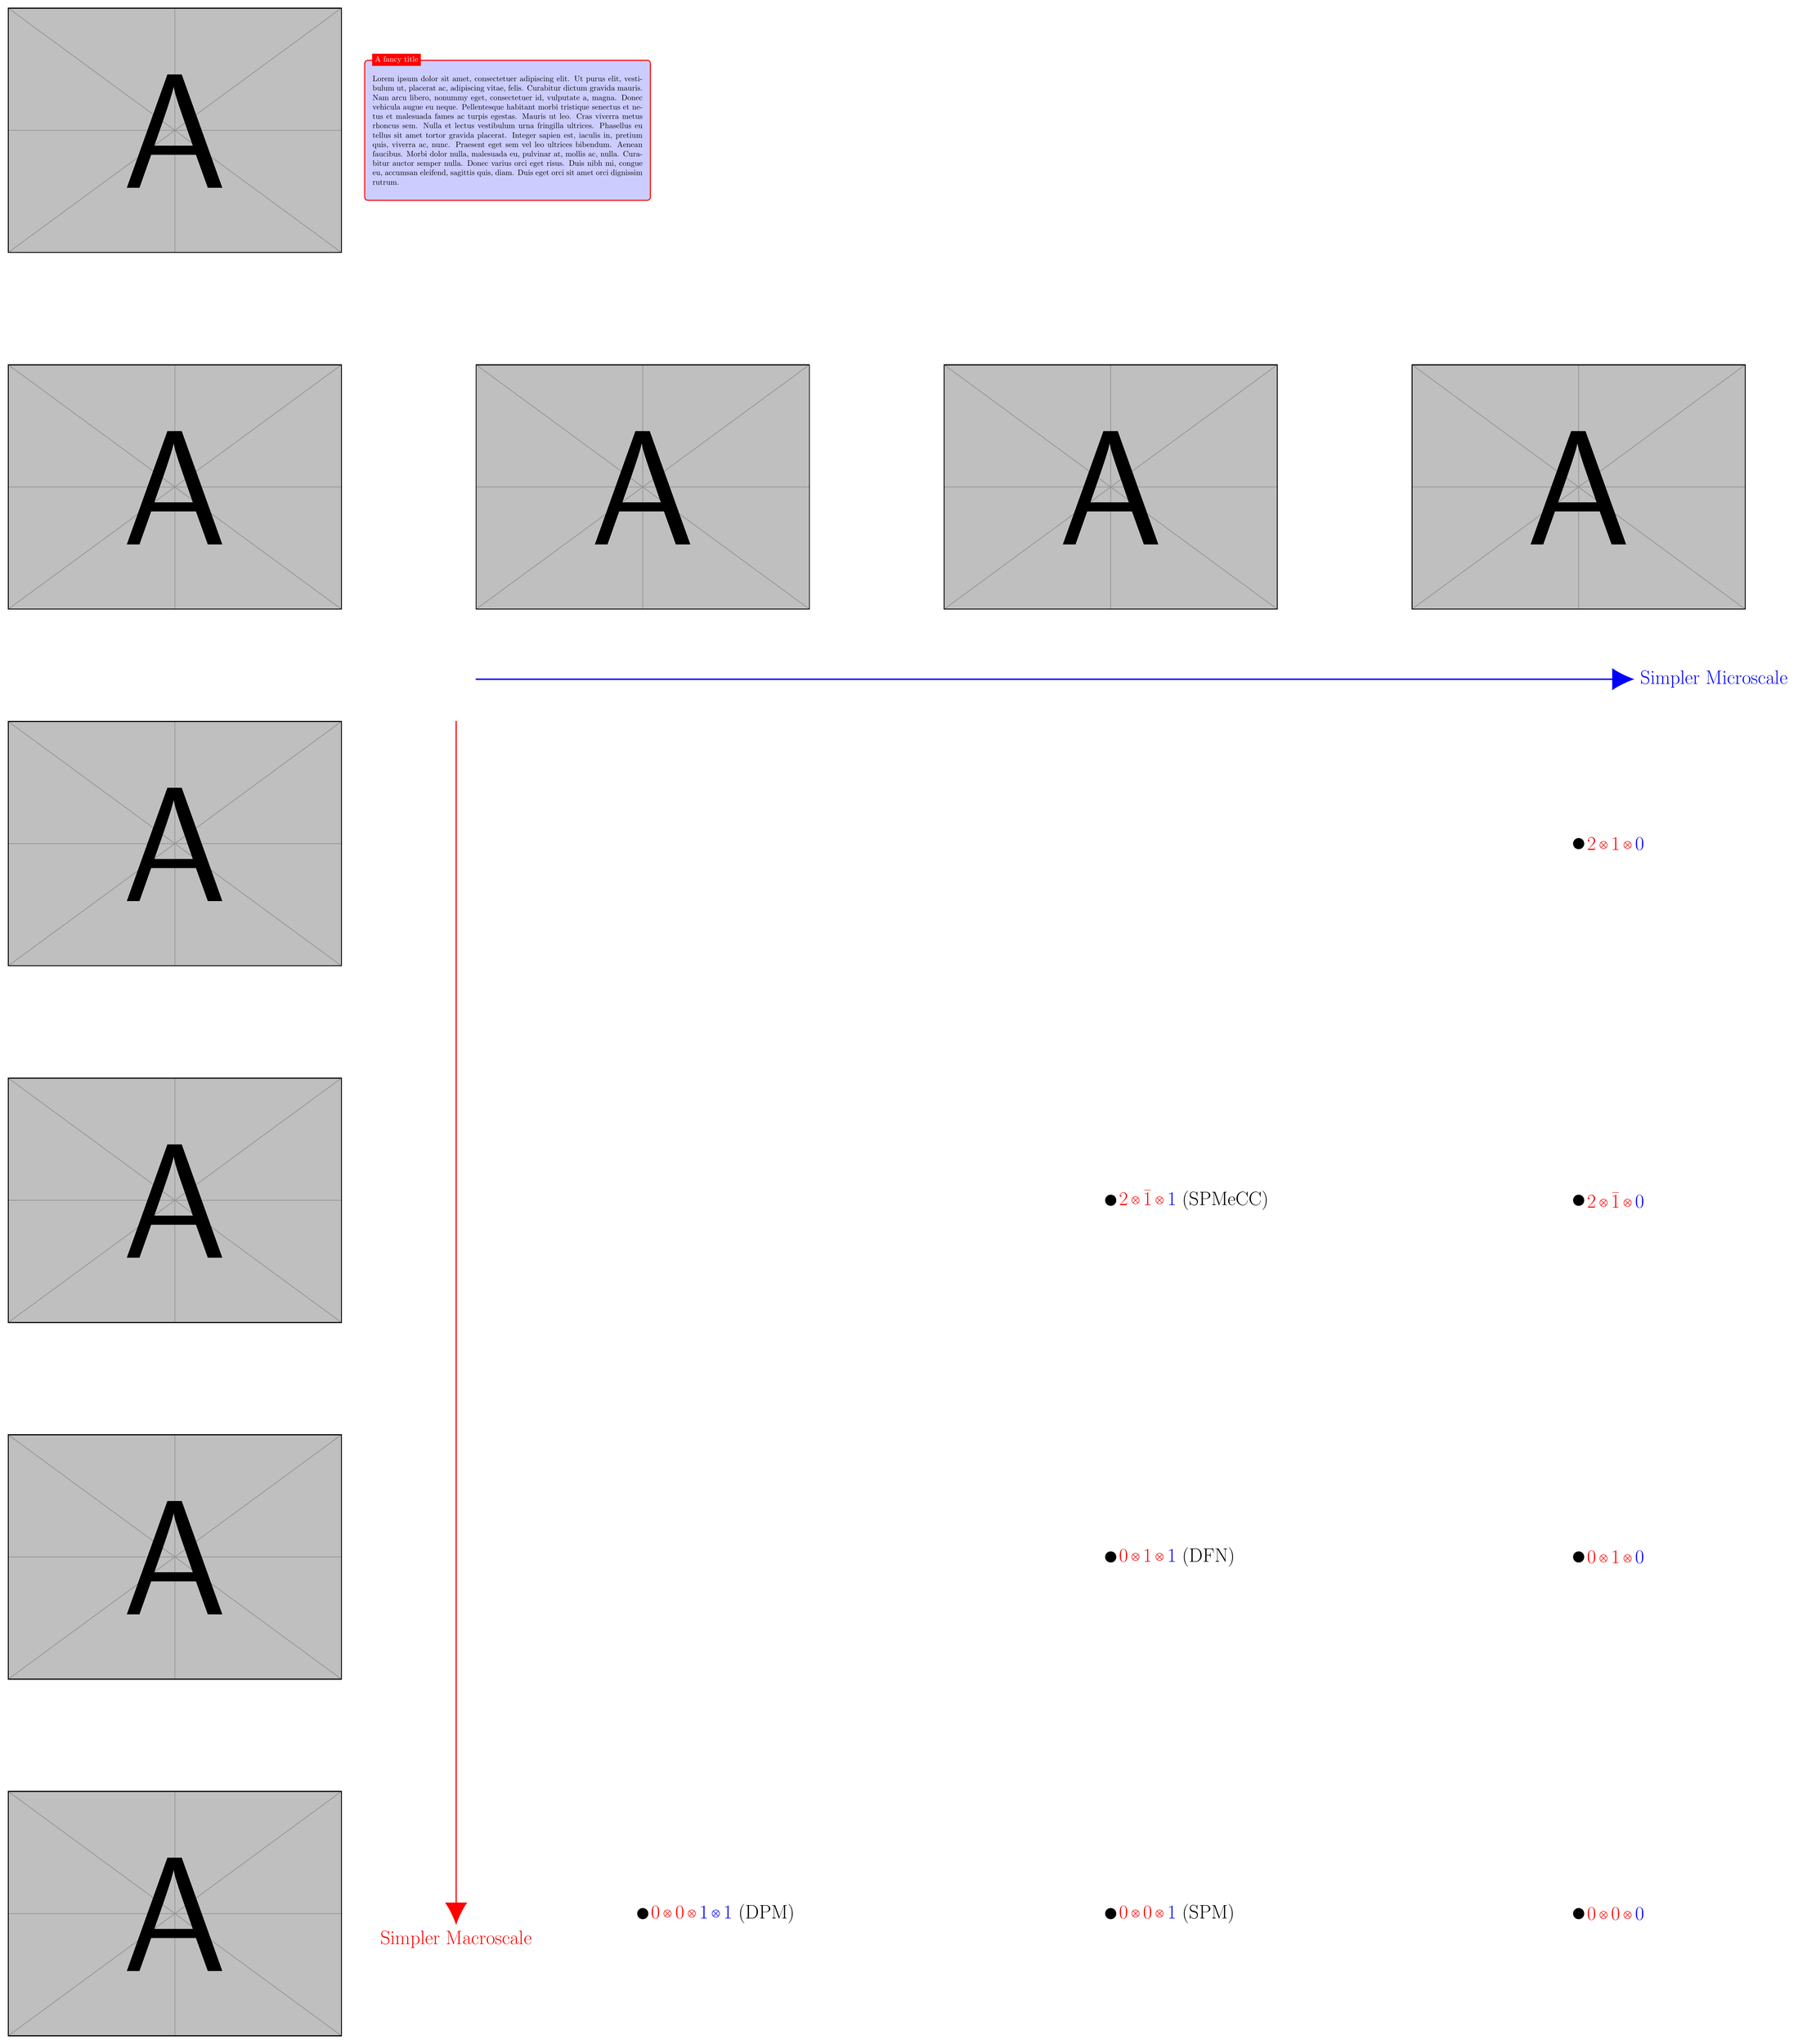
\begin{tikzpicture}
	% Grid lines (comment out to turn off)
	% \draw[help lines,color=black,xstep=1,ystep=1] (0,0) grid (80,90);
	% \foreach \x in {0,1,...,24} { \node [anchor=north] at (\x,0) {\x}; }
	% \foreach \y in {0,1,...,29} { \node [anchor=east] at (0,\y) {\y}; }

	% Full 3D
	\node [axisbox, anchor=north west](3d_full) at (0,90) {\includegraphics[width=\FIGWIDTH, height=\FIGHEIGHT]{example-image-a}};

	% 3 + 3
	\node [axisbox, below = \VERTFIGSEP of 3d_full, anchor=north](3_plus_3) {\includegraphics[width=\FIGWIDTH, height=\FIGHEIGHT]{example-image-a}};

	% Microscale row and axis
	\node [axisbox, right = \HORFIGSEP of 3_plus_3, anchor=west](3_plus_1_plus_1) {\includegraphics[width=\FIGWIDTH, height=\FIGHEIGHT]{example-image-a}};
	\node [axisbox, right = \HORFIGSEP of 3_plus_1_plus_1, anchor=west](3_plus_1) {\includegraphics[width=\FIGWIDTH, height=\FIGHEIGHT]{example-image-a}};
	\node [axisbox, right = \HORFIGSEP of 3_plus_1, anchor=west](3_plus_0) {\includegraphics[width=\FIGWIDTH, height=\FIGHEIGHT]{example-image-a}};
	% axis
	\node [below left = 3cm and 0cm of 3_plus_1_plus_1](x_axis_start) {};
	\node [below right = 3cm and -5cm of 3_plus_0](x_axis_end) {};
	\draw [axisline, \microcolor] (x_axis_start) -- (x_axis_end)
		node[right] {\Huge Simpler Microscale};

	% Text
	\node [mybox, right = of 3d_full] (box){%
    \begin{minipage}{\textwidth}
        \lipsum[1-1]
    \end{minipage}
	};
	\node[fancytitle, right=10pt] at (box.north west) {A fancy title};

	% Macroscale column and axis
	\node [axisbox, below = \VERTFIGSEP of 3_plus_3, anchor=north](2_plus_1_plus_3) {\includegraphics[width=\FIGWIDTH, height=\FIGHEIGHT]{example-image-a}};
	\node [axisbox, below = \VERTFIGSEP of 2_plus_1_plus_3, anchor=north](2_plus_1bar_plus_3) {\includegraphics[width=\FIGWIDTH, height=\FIGHEIGHT]{example-image-a}};
	\node [axisbox, below = \VERTFIGSEP of 2_plus_1bar_plus_3, anchor=north](0_plus_1_plus_3) {\includegraphics[width=\FIGWIDTH, height=\FIGHEIGHT]{example-image-a}};
	\node [axisbox, below = \VERTFIGSEP of 0_plus_1_plus_3, anchor=north](0_plus_0_plus_3) {\includegraphics[width=\FIGWIDTH, height=\FIGHEIGHT]{example-image-a}};
	% axis
	\node [above right = 0cm and 5cm of 2_plus_1_plus_3](y_axis_start) {};
	\node [below right = -5cm and 5cm of 0_plus_0_plus_3](y_axis_end) {};
	\draw [axisline, \macrocolor] (y_axis_start) -- (y_axis_end)
		node[below] {\Huge Simpler Macroscale};

	%%%%%%%%%%%%%%%%%%%%%%%%%%%%%%%%%%%%%%%%%%%%%%%%%%%%%%%%%%%%%%%%%%%%%%%%%%%%%%%%%%%%%%
	% Inner plot %%%%%%%%%%%%%%%%%%%%%%%%%%%%%%%%%%%%%%%%%%%%%%%%%%%%%%%%%%%%%%%%%%%%%%%%%
	%%%%%%%%%%%%%%%%%%%%%%%%%%%%%%%%%%%%%%%%%%%%%%%%%%%%%%%%%%%%%%%%%%%%%%%%%%%%%%%%%%%%%%
	% 2D+1D models
	\node [modelpoint,label=right:{$\macrotext{2\xo1}\xo\microtext{0}$}]
		at (2_plus_1_plus_3 -| 3_plus_0) {};
	\node [modelpoint,label=right:{$\macrotext{2\xo\bar{1}}\xo\microtext{1}$ (SPMeCC)}]
		at (2_plus_1bar_plus_3 -| 3_plus_1) {};
	\node [modelpoint,label=right:{$\macrotext{2\xo\bar{1}}\xo\microtext{0}$}]
		at (2_plus_1bar_plus_3 -| 3_plus_0) {};

	% Distributed particle models
	\node [modelpoint,label=right:{$\macrotext{0\xo0}\xo\microtext{1\xo1}$ (DPM)}]
		at (0_plus_0_plus_3 -| 3_plus_1_plus_1) {};

	% DFN, SPMe, SPM
	\node [modelpoint,label=right:{$\macrotext{0\xo1}\xo\microtext{1}$ (DFN)}]
		at (0_plus_1_plus_3 -| 3_plus_1) {};
	\node [modelpoint,label=right:{$\macrotext{0\xo0}\xo\microtext{1}$ (SPM)}]
		at (0_plus_0_plus_3 -| 3_plus_1) {};

	% Fast diffusion models
	\node [modelpoint,label=right:{$\macrotext{0\xo1}\xo\microtext{0}$}]
		at (0_plus_1_plus_3 -| 3_plus_0) {};
	\node [modelpoint,label=right:{$\macrotext{0\xo0}\xo\microtext{0}$}]
		at (0_plus_0_plus_3 -| 3_plus_0) {};
\end{tikzpicture}

\end{document}
